\chapter{DQN算法及其三大改进}
\section{Q-learning}
\subsection{马尔科夫决策过程}
\begin{defn}[马尔科夫性]
  当一个随机过程在给定现在状态及所有过去状态情况下,其未来状态的条件概率分布仅依赖于当前状态。A state $S_t$ is Markov if and only if :
  \begin{equation}
    P[S_{t+1}|S_t]=P[S_{t+1}|S_1,...,S_t]
  \end{equation}
\end{defn}

\begin{defn}[马尔科夫过程]
  马尔科夫过程即具有马尔科夫性的过程,即过程的条件概率仅仅与系统的当前状态相关,与它的未来或者过去历史都是独立不相关的。
\end{defn}
\begin{defn}[马尔科夫奖赏过程]
  相比于马尔科夫过程,马尔科夫奖赏过程(MRP)新增了转换过程中的奖赏函数,可以用四元组$<S,P,R,\gamma>$表示。
  \begin{itemize}
    \item $S$:有限状态的集合。
    \item $P$:表示不同状态之间相互进行转换的关系,可以用公式$P_{ss'}=P[S_{t+1}=s'|S_{t}=s]$来表示。
    \item $R$:奖赏函数。
    \item $\gamma$:折扣系数(discount factor)客观反映了更加看重眼前利益的特点,其中$\gamma$的范围为0~1闭区间。
  \end{itemize}
  \begin{defn}[奖赏函数]
    在$t$时刻的奖赏值$G_t$:
    \begin{equation}      
      G_t=R_{t+1}+\gamma R_{t+2}+...=\sum_{k=0}^\infty \gamma^k R_{t+k+1}
    \end{equation}
  \end{defn}
\end{defn}

为什么需要折扣系数$\gamma$:
\begin{itemize}
  \item 方便数学表达。
  \item 避免陷入无限循环。
  \item 长远利益有不确定性。
  \item 立即的回报相对于延迟的回报能获得更多利益。
  \item 符合人类更看重眼前利益的特点。
\end{itemize}
\begin{defn}[价值函数]
  状态$s$的长期价值函数表示为:
  \begin{equation}
    v(s)=E[G_t|S_t=s]
  \end{equation}
\end{defn}

\begin{defn}[马尔科夫决策过程]
  相比于马尔科夫奖赏过程,马尔科夫决策过程(Markov Decision Process,MDP)新增了在状态s下执行动作的决策函数,MDP可以使用五元组$<S,A,P,R,\gamma>$来表示。
  \begin{itemize}
    \item $S$:有限状态的集合。
    \item $A$:有限动作的集合。
    \item $P$:表示不同状态之间相互进行转换的关系,可以用$P_{ss^{'}}^a=P[S_{t+1}=s^{'}|S_t=s,A_t=a]$来表示。
    \item $R$:奖赏函数。
    \item $\gamma$:折扣系数(discount factor)客观反映了更加看重眼前利益的特点,其中$\gamma$的范围为0~1闭区间。
  \end{itemize}
\end{defn}

\begin{defn}[策略]
  给定状态下的动作概率分布:
  \begin{equation}
    \pi(a|s)=P[A_t=a|S_t=a]
  \end{equation}  
\end{defn}
\begin{defn}[状态价值函数]
  在处于某一环境中,机器自身的策略$\pi$的情况下,当机器在环境中处于状态s时,此时s自身存在一个价值,可以用价值函数来表示:
  \begin{equation}
    v_{\pi}(s)=E_{\pi}[G_t|S_t=s]
  \end{equation}
\end{defn}
\begin{defn}[最优状态价值函数]
  在处于某一环境中,机器自身的策略$\pi$的情况下,当机器在环境中处于状态s时,此时s自身存在的最优状态价值函数为:
  \begin{equation}
    v_{*}(s)=\max_{\pi}v_{\pi}(s)
  \end{equation}
\end{defn}
\begin{defn}[动作价值函数]
  在处于某一环境中,机器自身的策略为$\pi$、环境当前的状态为$s$的情况下,机器执行某一动作$a$会产生一定量的价值,这种价值和策略、状态、动作的关系可以表示为:
  \begin{equation}
    q_{\pi}(s,a)=E_{\pi}[G_t|S_t=s,A_t=a]
  \end{equation}
\end{defn}
\begin{defn}[最优动作价值函数]
  状态$s$下采取动作$a$的最优动作价值函数:
  \begin{equation}
    q_{*}(s,a)=\max_{\pi}Q_{\pi}(s,a)
  \end{equation}
\end{defn}
\begin{defn}[最优策略]
  如果策略$\pi$优于策略$\pi^{'}$:
  \begin{equation}
    \pi \geq \pi^{'} , if: v_{\pi}(s) \geq v_{\pi^{'}}(s),\forall_{s}
  \end{equation}
    
\end{defn}

\subsection{Q-learning}
对于任何马可尔夫决策过程,Q-learning\cite{Mnih2013Playing}是当前状态的最佳策略。
Q-learning通过Q估计进行决策,通过Q现实进行更新。
\begin{defn}[Q 估计]
  在当前状态s下做出动作a后到达的状态s\_获得的奖励的估计值。
\end{defn}
\begin{defn}[Q 现实]
  在当前状态s下做出动作a后到达状态s\_获得的奖励的实际值。
\end{defn}
\begin{defn}[Q 表]
  当机器在环境中处于不同的状态$s_i$下,执行不同的动作$a_j$时,会产生不同且唯一确定的价值Q,把所有的状态与执行动作的组合得到的价值列成一张表格,称之为Q表(Q-table)。
  \begin{table}
    \begin{center}
      \caption{Q-table}
      \begin{tabular}{|l|c|r|} 
        \hline
        Q-table & $a_1$ & $a2$ \\ 
        \hline
        $s_1$ & $Q(s_1,a_1)$ & $Q(s_1,a_2)$ \\ 
        \hline
        $s_2$ & $Q(s_2,a_1)$ & $Q(s_2,a_2)$ \\ 
        \hline
        $s_3$ & $Q(s_3,a_1)$ & $Q(s_3,a_2)$ \\ 
        \hline
      \end{tabular}
      
    \end{center}
  \end{table}
  
\end{defn}
Agent(玩家)进入每个状态$s_i$时,通过查阅Q表,能得到在$s_i$时选择不同动作$a_i$的期望值(Q 估计)$Q(s_i,a_i)$,选择其中最大的Q值所对应的动作,会进入不同的状态$s_j$,同时环境会给agent一个回报reward(Q 现实)。
\begin{cor}[Q-learning]
  根据以上推导,可以对Q值计算,也就是Q\_table更新过程,其中$\alpha$为学习率,$\gamma$为奖励性衰变系数。
  \begin{equation}
    Q\left(S_{t}, A_{t}\right) \leftarrow Q\left(S_{t}, A_{t}\right)+\alpha\left[R_{t+1}+\gamma \max _{a} Q\left(S_{t+1}, a\right)-Q\left(S_{t}, A_{t}\right)\right]
  \end{equation}
\end{cor}
\begin{exmp}[挖宝藏小游戏]
  
  O - - - - T

  在这个例子中,O代表agent,T代表宝藏,一开始宝藏在最右边,agent在最左边,在每一步动作中,agent可以选择两个动作,left(向左走)或者right(向右走)。

  例如,在这个过程中的某个状态为:

  - O - - - T

  接下来Agent可以选择
  \begin{itemize}
    \item left:O - - - - T
    \item right:- - O - - T
  \end{itemize}

  我们可以用O所在的位置(0,1,2,3,4,5)表示agent所在的状态,当agent比上一个状态更加靠近宝藏的时候,我们(环境)给agent一个正反馈(reward>0),当agent比上一步远离agent的时候,我们给agent一个负反馈(reward<0)。

  那么此时的Q表为如下形式:
  \begin{table}
    \begin{center}
      \caption{挖宝藏小游戏 Q-table}
      \begin{tabular}{|l|c|r|}
        \hline
        $Q-table$ & left & right \\
        \hline
        0 & q(0,left) & q(0,right) \\
        \hline
        1 &q(1,left) &q(1,right) \\
        \hline
        2 &q(2,left)  &q(2,right) \\
        \hline
        3 &q(3,left) &q(3,right) \\
        \hline
        4 &q(4,left) &q(4,right) \\
        \hline
        5 &q(5,left) &q(5,right) \\
        \hline
      \end{tabular}
    \end{center}
  \end{table}

  当Agent在i位置的时候,当Agent选择$right$,Agent将会靠近宝藏,那么Agent将会获得环境的正反馈$r_i$,那么对应的$Q(i,right)$将会增加$r_i$;如果Agent选择$left$,那么Agent会远离宝藏,环境会给Agent一个负反馈$r_i$,那么对应的$Q(i,right)$将会减少$r_i$。

\end{exmp}

通过智能体(Agent)、环境(environment)、奖励(reward)、动作(action),状态(state)这五个要素可以将问题抽象成一个马尔科夫决策过程,我们在每个格状态$s_t$可以根据Q\_table选择一个动作执行,得到环境状态的反馈同时进入下一个状态$s_{t+1}$,根据环境反馈的状态更新Q\_table。
\cleardoublepage
\begin{algorithm}
  \caption{Q-learning}
  \label{Q-learning}
  \begin{algorithmic}[1]
    \State {初始化$Q-table$}
    \For{回合 $in$ 所有回合}
    \State 初始化状态s
    \For{步骤 $in$ 本回合所有步骤}
    \State 使用$Q-table$在当前状态$s$所有可以选择的$action$中,选取$Q$值最大的动作$a$
    \State 执行动作$a$,获得环境反馈的奖励值$r$,并进入新的状态$s^{'}$
    \State 更新$Q-table$ : $$Q\left(S_{t}, A_{t}\right) \leftarrow Q\left(S_{t}, A_{t}\right)+\alpha\left[R_{t+1}+\gamma \max _{a} Q\left(S_{t+1}, a\right)-Q\left(S_{t}, A_{t}\right)\right]$$
    \State $s \gets s'$
    \EndFor
    \EndFor
  \end{algorithmic}
\end{algorithm}

传统强化学习Q-learning算法通过一张Q-table不断探索和更新Q值,计算出agent最佳的选择。Q-table必须把agent可能遇到的每一个状态都存下来,那么在面对如电子游戏这样的复杂游戏下,状态数量过多,Q-table将会大到无法想象,计算机无法存储如此大表格。因此传统强化学习Q-learning无法处理这样的复杂环境。
\section{卷积神经网络}
深度学习自从2006年以来受到了广泛的关注,目前深度学习已经成为大数据(Big Data)和人工智能(AI)的一个研究热点。通过建立起类似于人脑的神经网络结构,深度学习神经网络可以提取出输入数据从低层次到高层次的特征,很好的建立起了底层原始输入信号到高层语义理解的映射关系。
深度学习可以表示多层次抽象的数据(如知识图谱,词向量),用来提供给不同的计算模型进行学习任务。深度学习这种方法在许多领域都引领了发展,包括最先进的语音识别、计算机视觉对象识别、对象检测和许多其它领域如医疗领域等。大数据中的复杂结构可以通过深度学习来进一步挖掘和发现,BP算法能够指导计算机从后面的神经网络层传递误差到前面的神经网络层来改变本层的参数。在计算机视觉领域的处理、语音合成、音频处理等方面,深度学习已经有了较为成熟的工业应用,而神经网络中的一种网络结构递归网络,在文本和语音等处理序列的方面展现了强大的能力。
\subsection{基本概念}
\begin{defn}[人造神经元(Neuron)]
  类似于人类大脑的基本单元,大量的神经元排列组合构成了神经网络。在神经网络中,神经元接收输入数据,经过神经元的处理得到输出,而这个输出被发送到其他神经元用于进一步处理,或者作为最终输出进行输出。 
  一般神经元包含:
  \begin{itemize}
    \item 输入:神经元的输入数据;
    \item 权重:当输入进入神经元时,它会乘以一个权重;
    \item 偏差:改变权重与输入相乘所得结果的范围;
    \item 激励函数:决定了当前神经元是否达到激活状态,通常为非线性函数如Sigmoid,Relu等;
    \item 输出:神经元的输出数据。
  \end{itemize}
  数学表示:$t=f(W*A+b)$,W为权重向量,A为输入向量,b为偏置,f为激励函数,t为输出。
  
\end{defn}
\begin{figure}[ht]
  \centering
  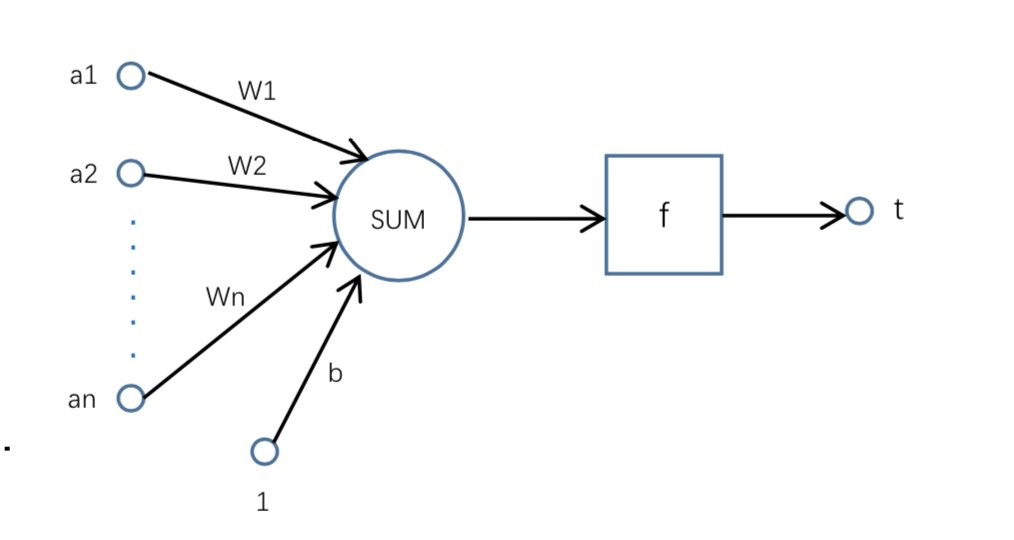
\includegraphics[scale=0.4]{static/Ncell.png}
  \caption{人造神经元}
\end{figure}

\begin{defn}[神经网络]
  神经网络是由大量神经元经过不同的排列组合而形成,不同的神经元之间之间传递相互数据,通过BP算法来不断调整自身的参数。神经元具有激活阈值,相当于神经元激活的最低要求值,如果神经元的权重值的组合和传递给它的数据之和大于等于这个阈值的话,将会导致神经元产生激活,神经元的组合可以产生学习的能力。
  典型的人工神经网络具有以下三个部分:
  \begin{itemize}
    \item 结构,结构指定了网络中的变量和它们的拓扑关系;
    \item 激励函数,定义了神经元改变自身状态(是否激活)的规则,如果激活就可以将数据传递到下一层,一般是一个非线性函数;
    \item 学习规则,学习规则指定了网络中的权重参数如何随着时间推进而进行相应的调整。
  \end{itemize}
  
\end{defn}

\begin{figure}
  \centering
  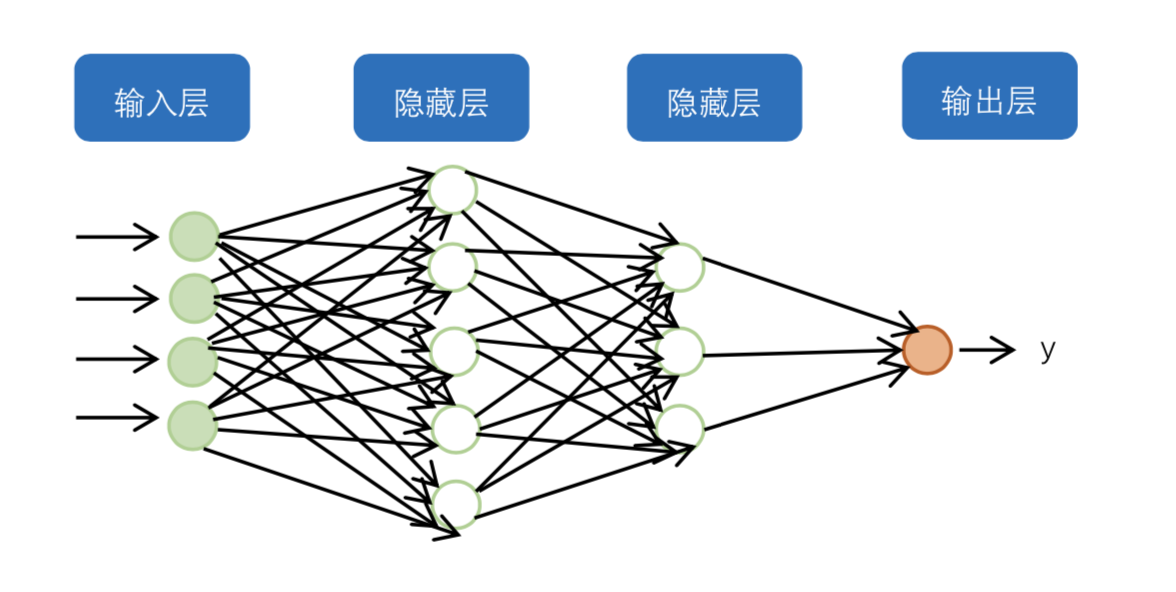
\includegraphics[scale=0.5]{static/network.png}
  \caption{普通神经网络}
\end{figure}

\begin{defn}[输入层]
  接受输入的那一层,本质上是网络的第一层;
\end{defn}
\begin{defn}[输出层]
  生成输出的那一层,本质上是网络的最后一层;
\end{defn}
\begin{defn}[隐藏层]
  处理输入层传入的信号的中间若干层的神经网络,隐藏层根据不同的任务做不同的处理得到中间输出数据,传递到下一层。
\end{defn}
\subsection{多层神经网络}
\begin{defn}[MLP(多层感知器)]
  单个神经元能执行的任务(函数)复杂度有限,类似于CPU中的门结构,使用大量神经元进行堆栈组合可以实现复杂任务的处理输出。一个输入层、一个隐藏层和一个输出层可以构成最简单的神经网络。每个层都有多个神经元,并且每个层中的所有神经元都连接到下一层的所有神经元。这些网络也可以被称为完全连接的网络。 
\end{defn}
多层神经网络的学习过程
\begin{enumerate}
  \item 从输入层开始,原始输入数据通过神经网络向前传递,数据经过不同层次的处理得到输出结果;
  \item 基于网络的输出,通过损失函数得到目标与当前数据的误差;
  \item 反向计算这个误差,计算误差相对于网络中每个权值参数的导数,更新模型的参数。
\end{enumerate}
2006年,深度学习的经典文章《Reducing the dimensionality of data with neural networks》\cite{hinton2006reducing}提出了如下的主要观点:
\begin{enumerate*}
  \item 多层神经网络具有更加优异的特征学习能力;
  \item 通过逐层初始化可以有效克服多层神经网络更新学习的困难。
\end{enumerate*}

\subsection{卷积神经网络}

卷积神经网络(Convolutional Neural Networks, CNN)是一种特殊的神经网络结构,包含了若干个卷积层和池化层,以此完成对原始数据特征的抽取。不同于普通神经网络中的全连接,在卷积层中,一个神经元只与部分相邻网络层中的神经元进行连接。通过卷积和子采样(池化)两个操作可以大大简化模型复杂度,减少模型需要调整的参数。
\begin{figure}[h]
  \centering
  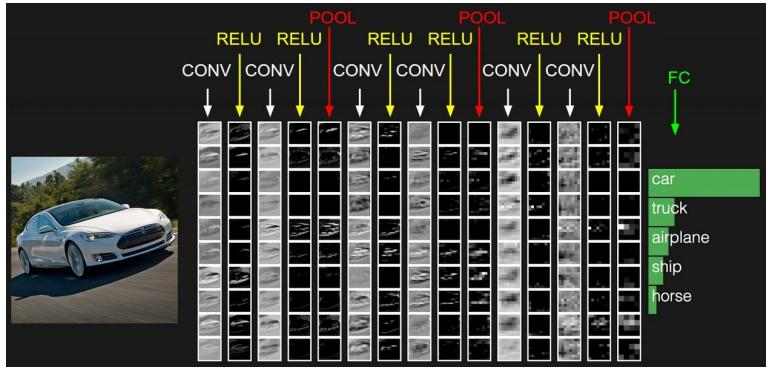
\includegraphics[scale=0.5]{static/cnn.jpg}
  \caption{典型卷积神经网络结构\cite{CNN2017}}
\end{figure}
卷积神经网络是传统神经网络的一个改进,在普通层级神经网络的基础上对不同层的功能和形式做出了一些改变。
卷积神经网络的一般结构:
\begin{enumerate}
  \item 数据输入层/ Input layer
  \item 卷积计算层/ CONV layer
  \item 激励函数层 / ReLU layer
  \item 池化层 / Pooling layer
  \item 全连接层 / FC layer
\end{enumerate}


数据输入层主要是对原始图像数据进行预处理,其中包括:
\begin{itemize}
  \item 去均值操作:为了把样本的中心拉回到坐标系原点上,对输入的原始数据在各个维度上都中心化为0;
  \item 归一化: 为了减少各个维度数据取值差异带来的干扰,将不同维度的数据范围归一化相同的范围,如将原始所有的数据归一化到[-1,1]的范围;
  \item 白化:相当于在数据的特征轴上对数据做归一化。
\end{itemize}

卷积层是卷积神经网络最重要的一个层次,
在卷积层中,有两个关键操作:
\begin{itemize}
  \item 窗口滑动,滤波器对局部数据进行计算,提取出数据的局部特征;
  \item 局部关联,将神经元视为滤波器,使用神经元对原始数据做滤波操作。 
\end{itemize}

卷积神经网络采用的激励函数一般为ReLU(The Rectified Linear Unit,修正线性单元),通过这样的非线性函数可以将卷积层的输出结果做非线性映射。
采取Relu可以加速网络的收敛,方便求网络的梯度,函数的图像如(\ref{fig:Relu})所示:
\begin{figure}[h]
  \centering
  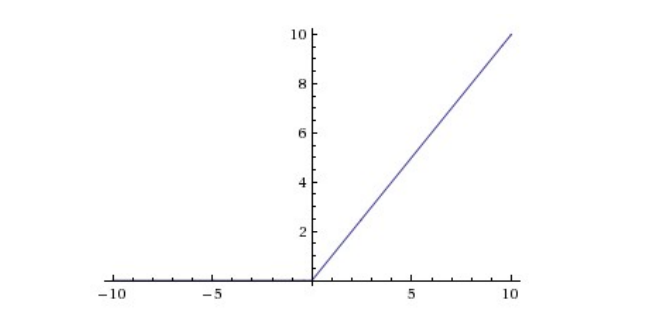
\includegraphics[scale=0.5]{static/Relu.png}
  \caption{Relu函数图像}
  \label{fig:Relu}
\end{figure}

为了压缩数据和减少参数的数量,减小神经网络过拟合的风险,可以通过池化操作完成。池化层位于连续的卷积层中间,
具体来说,如果输入是图像数据的话,那么池化层的最主要作用就是压缩图像的大小。

卷积神经网络尾部一般用全局连接层来进行连接过渡,和普通的神经网络神经元的连接方式完全相同。全连接层一般用于得出神经网络最后的输出结果。
\section{DQN算法}
伴随着深度学习的发展,深度学习也在传统强化学习产生重要的应用,DQN(deep Q network)就是一种融合了深度学习与强化学习的方法。

2015年DeepMind在文章《Playing Atari with Deep Reinforcement Learning》\cite{mnih2013playing}提出了DQN ,DQN是第一个直接从图像的原始像素中成功学习到控制策略的深度强化学习算法。DQN使用卷积神经网络代替Q-learning中的价值函数,对机器当前状态应选的动作输出相应的动作价值。因此DQN算法的决策核心就是卷积神经网络,DQN的输入为原始图像像素,输出为当前状态的价值函数,训练采用Q-learning的方法来进行。DQN算法应用到Atari2600的许多游戏上,取得很大的成功,有的甚至达到了超越人类最高分的水平。

之后DeepMind在Nature上发表了改进版的DQN文章\cite{mnih2015human},引起了广泛的关注,深度强化学习从此成为深度学习领域的前沿研究方向与研究热门。

将深度学习应用在强化学习上,面临诸多挑战。大部分深度学习算法需要巨大的训练数据量,但传统强化学习提供的数据通常比较稀疏,噪声也很大,通常在执行完动作不能立即获得奖励;强化学习获得的回报与产生这个结果的动作可能会有很长的间隔,各个相邻的状态之间有很强的关联性,而深度学习一般假设样本数据独立进行分布。就是,随着训练的进程,价值函数对动作价值的估计不断得到优化。而随着价值函数的变化,其Q值输出(动作输出)也会跟着改变,继而产生的训练样本的分布也会改变,这与深度学习要求训练用的数据分布不变不符合。

DQN不用Q表记录Q值,而是用神经网络来预测Q值,并通过不断更新神经网络从而学习到最优的行动路径。
DeepMind 用DQN来玩电子游戏,他们将游戏画面的像素转换成深度神经网络的输入数据(状态s),用CNN(卷积神经网络)来预测动作a($a_1$,$a_2$,$a_3$ ....), 和对应的Q(s, $a_1$), Q(s, $a_2$),Q(s, $a_3$)...
然后算法通过更新神经网络(NN)中的参数(w, b ...),来更新NN,从而优化模型得到最优解。

为了使训练的样本之间不会相互依赖,DQN设置了一个经验库用来存放以前不同状态之间的转换关系的数据,然后每次在经验库中经过随机采样得到训练所需的数据样本;采用过去的多个样本做平均,训练样本分布得到平滑,使得样本分布变化的问题得到减缓。
在经验回放过程中,将多个回合转化过程中,机器每一步使用神经网络贪心地选择动作,产生的经验$e_t = <s_t, a_t, r_t, st+1>$,存入一个经验记忆池D中。在算法参数更新的操作中,对记忆池里的样本数据进行随机采样或批量随机采样,通过Q-learning算法对模型进行参数更新。由于神经网络无法处理边长的原始数据,因此DQN使用固定长度的历史数据表示状态,例如过去连续若干图像帧的排列。

DQN这种方法对于传统的在线Q-learning来说,具有以下优势:
\begin{itemize}
  \item 通过多次采样每一步的数据,很大程度上提高了数据的利用效率。
  \item 通过随机采样打破了从连续数据里学习效率低下的问题,降低更新参数的方差。
  \item 通过在经验库中随机采样,可以得到平均分布的各个状态下的数据,解决了训练会产生发散的问题。
\end{itemize}

\begin{figure}[h]
  \centering
  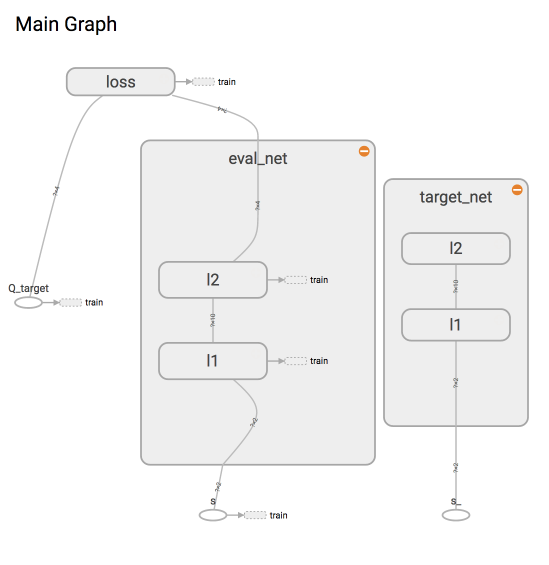
\includegraphics[scale=0.5]{static/dqn.png}
  \caption{DQN网络结构}
\end{figure}
DQN中的损失函数定义为:
\begin{equation}
  \label{DQN:loss}
  L_{i}\left(\theta_{i}\right)=\mathbb{E}_{s, a \sim \rho(\cdot)}\left[\left(y_{i}-Q\left(s, a ; \theta_{i}\right)\right)^{2}\right]
\end{equation}


DQN中有两个神经网络。一个参数相对固定的网络,我们叫做target-net,用来获取Q-目标(Q-target)的数值, 另外一个叫做eval-net用来获取Q-评估(Q-eval)的数值。
我们在训练神经网络参数时用到的损失函数(Loss function),实际上就是q\_target 减 q\_eval的结果 (loss = q\_target- q\_eval )。
反向传播真正训练的网络是只有一个,就是eval\_net。target\_net 只做正向传播得到q\_target $(q\_target = r +\gamma*max Q(s,a))$. 其中 Q(s,a)是若干个经过target-net正向传播的结果。

训练的数据是从记忆库中随机提取的,记忆库记录着每一个状态下的行动,奖励,和下一个状态的结果$<s, a, r, s^{'}>$。记忆库的大小有限,当记录满了数据之后,下一个数据会覆盖记忆库中的第一个数据,记忆库就是这样覆盖更新的。
q\_target的网络target\_net也会定期更新一下参数,由于target\_net和eval\_net的结构是一样的。更新q\_target网络的参数就是直接将q\_eval 的参数复制过来。
\cleardoublepage
\begin{algorithm}
  \caption{DQN算法}
  \begin{algorithmic}
    \State 初始化检验回放库D大小为N
    \State 初始化Q网络参数
    \For{i in range(回合总数M)}
    初始化状态$s_1=\{x_1\}$,并预处理$\phi_1=\phi\{s_1\}$
    \For{t in range(T)}
    \State 通过概率分布为$\epsilon$ 的概率,选取当前一个动作$a_t$
    \State 否则选取动作$a_t=\max_a Q^* (\phi(s_t),a;\theta)$
    \State 执行动作$a_t$,并获得获得环境给的反馈$r_t$,进入新的画面$x_{t+1}$
    \State 设置$s_{t+1}=s_t,a_t,x_{t+1}$并且处理$\phi_{t+1}=\phi(s_{t+1})$
    \State 将$(\phi_t,a_t,r_t,\phi_{t+1})$存储到经验库D中
    \State 从经验库D中随机抽取转换关系$(\phi_j,a_j,r_j,\phi_{j+1})$
    \If{$\phi_{j+1}$时刻游戏结束}
    \State $y_j=r_j$
    \Else
    \State $y_j=r_j+\gamma \max_{a^{'}}Q(\phi_j,q_j;\theta)$
    \EndIf
    \State 实施梯度下降更新网络参数,$loss=(y_j-Q(\phi_j,a_j;\theta))$
    \EndFor
    \EndFor
  \end{algorithmic}
\end{algorithm}

\section{DQN三大改进}
\subsection{double DQN}
double DQN\cite{van2016deep,hasselt2010double}的改进是关于DQN的公式的改进。
根据上面的损失函数(\ref{DQN:loss}),$y_i$也被我们称为q-target值,而后面的Q(s,a)我们称为q-eval值,我们希望q-target和q-eval值越接近越好。

q-target计算的公式:
\begin{equation}
  Y_{t}^{\mathrm{Q}} \equiv R_{t+1}+\gamma \max _{a} Q\left(S_{t+1}, a ; \boldsymbol{\theta}_{t}\right)
\end{equation}
进一步展开:
\begin{equation}
  Y_{t}^{\mathrm{Q}}=R_{t+1}+\gamma Q\left(S_{t+1}, \underset{a}{\operatorname{argmax}} Q\left(S_{t+1}, a ; \boldsymbol{\theta}_{t}\right) ; \boldsymbol{\theta}_{t}\right)
\end{equation}

也就是说,我们根据状态$s^{'}$选择动作$a^{'}$的过程,以及估计Q($s^{'}$,$a^{'}$)使用的是同一张Q值表,或者说使用的同一个网络参数,这可能导致选择过高的估计值,从而导致过于乐观的值估计。

为了避免这种情况的出现,我们可以对选择和衡量进行解耦,从而就有了doubel DQN,在Double DQN中,q-target的计算基于如下的公式:
\begin{equation}
  \label{alg:double-dqn}
  Y_{t}^{\text { DoubleQ }} \equiv R_{t+1}+\gamma Q\left(S_{t+1}, \operatorname{argmax}_{a} Q\left(S_{t+1}, a ; \boldsymbol{\theta}_{t}\right) ; \boldsymbol{\theta}_{t}^{\prime}\right)
\end{equation}

我们根据一张Q表或者网络参数来选择我们的动作$a^{'}$,再用另一张Q值表活着网络参数来衡量Q($s^{'}$,$a^{'}$)的值。
\subsection{Prioritized Experience Replay DQN}
Prioritized Experience Replay DQN\cite{,schaul2015prioritized} 是关于DQN在经验回放的改进。
对于增强学习过程中,agent在一系列的动作选择中得到的经验,存在很大的相关性,这违反了常见的梯度下降算法对于样本的假设。同时对于一些出现几率很小,但是可能很有用的经验,忘记得非常快。
经典DQN在经验回放学习时采取均匀采样的方法,那么当一个agent在学习过程中,遇到的正例很少,负例很多的类似正反馈负反馈样本及其不均衡的时候,那么agent每一次回放学习到的东西就会非常少,学习效率就会变得十分低下。

DQN使用了experience replay(经验回放)来克服这些困难。
对于prioitization(优先级),重要的是如何衡量经验的重要性。作者选择了TD-error(\ref{TD-error})(Temporal-Difference error,时序差分-error)。它直观地解释是:agent对这个经验的惊讶程度,也就是有多超乎意料。
如果 TD-error 越大, 就代表我们的预测精度还有很多上升空间, 那么这个样本就越需要被学习, 也就是优先级 p 越高.
TD-error:
\begin{equation}\label{TD-error}
  \delta_{t} :=R_{t}+\gamma_{t} \max _{a} Q\left(S_{t}, a\right)-Q\left(S_{t-1}, A_{t-1}\right)
\end{equation}
在这篇论文中,作者提出来优先选择那些对于训练更加有效的经验,而不是DQN中的随机提取经验进行学习。因为,对于一个agent来说,某些经验会比其他经验更加有用,对于那些TD-error更大的经验,给予更多的检验回放的机会。

有了 TD-error 就有了优先级 p, 那我们如何有效地根据 p 来抽样呢? 如果每次抽样都需要针对 p 对所有样本排序, 这将会是一件非常消耗计算能力的事。因此需要采取另一种方法, 这种方法不会对得到的样本进行排序。这种抽样方法就叫做SumTree。
\begin{figure}[h]
  \centering
  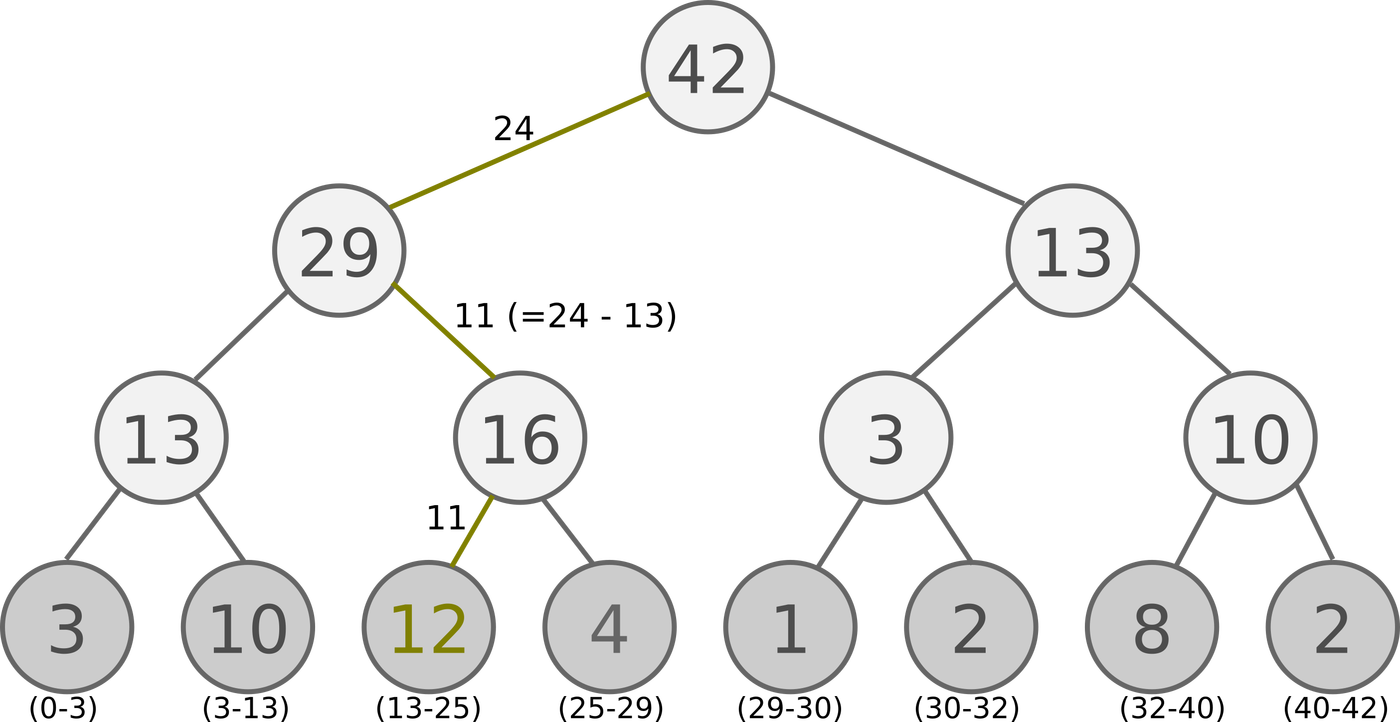
\includegraphics[scale=0.5]{static/sum_tree.png}
  \caption{SumTree}
\end{figure}
SumTree 是一种树形结构, 每片树叶存储每个样本的优先级 p, 每个树枝节点只有两个分叉, 节点的值是两个分叉的合, 所以 SumTree 的顶端就是所有 p 的合. 最下面一层树叶存储样本的 p, 叶子上一层最左边的 13 = 3 + 10, 按这个规律相加, 顶层的 root 就是全部 p 的和。

抽样时, 我们会将 p 的总合 除以 batch size, 分成 batch size 那么多区间, (n=sum(p)/batch\_size)。如果将所有 node 的 priority 加起来是42的话, 我们如果抽6个样本, 这时的区间拥有的 priority 可能是这样:
$$[0-7], [7-14], [14-21], [21-28], [28-35], [35-42]$$

然后在每个区间里随机选取一个数. 比如在第区间 [21-28] 里选到了24, 就按照这个 24 从最顶上的42开始向下搜索. 首先看到最顶上 42 下面有两个 child nodes, 拿着手中的24对比左边的 child 29, 如果 左边的 child 比自己手中的值大, 那我们就走左边这条路, 接着再对比 29 下面的左边那个点 13, 这时, 手中的 24 比 13 大, 那我们就走右边的路, 并且将手中的值根据 13 修改一下, 变成 24-13 = 11. 接着拿着 11 和 13 左下角的 12 比, 结果 12 比 11 大, 那我们就选 12 当做这次选到的 priority, 并且也选择 12 对应的数据.
\subsection{Dueling DQN}
一般来说在基于视觉感知的深度强化学习任务中,同一个状态下不同的动作会产生不一样的环境反馈,但在某些情况下环境的反馈与执行的动作无关。根据上面的思想,一种新的竞争网络结构被提出作为DQN的网络模型:Dueling Network。

用一句话来概括 Dueling DQN\cite{wang2015dueling} 就是. 它将每个动作的 Q 拆分成了 state 的 Value 加上 每个动作的 Advantage.

dueling DQN的q值由以下来确定
\begin{equation}
  Q(s, a ; \theta, \alpha, \beta)=V(s ; \theta, \beta)+A(s, a ; \theta, \alpha)
\end{equation}
它分成了这个 state 的值, 加上每个动作在这个 state 上的 advantage(优势值)。 因为有时候在某种 state,无论做什么动作,对下一个 state 都没有多大影响。
\begin{figure}[h]
  \centering
  \label{fig:dueling}
  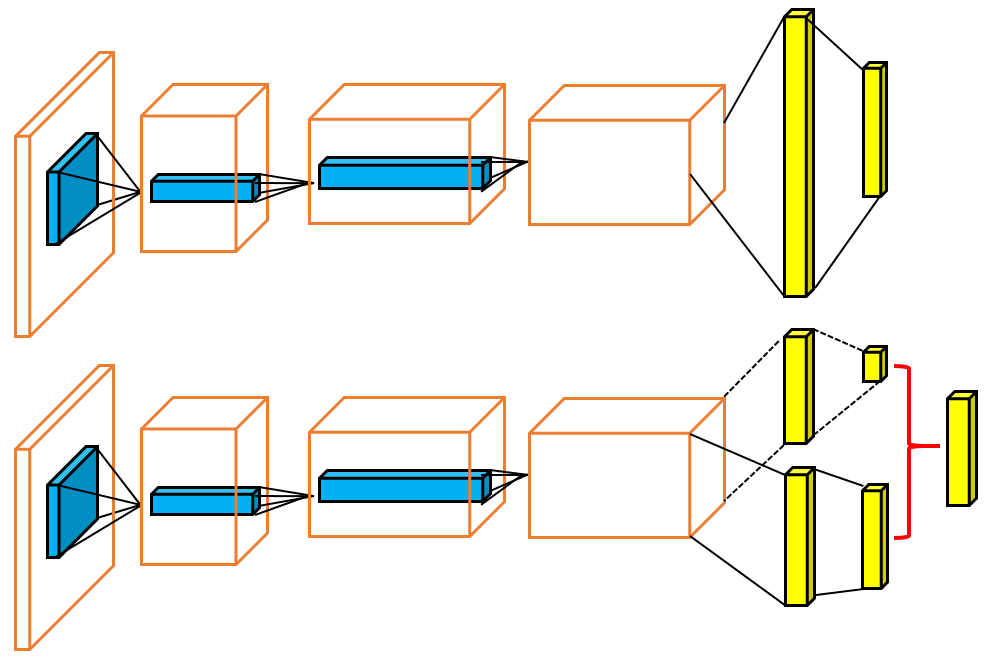
\includegraphics[scale=0.5]{static/dueling.png}
  \caption{普通网络结构与Dueling-Net结构}
\end{figure}

如下图所示,第一个模型为一般的DQN神经网络结构,第二个为Dueling-Net的网络结构。DQN网络结构输入层接入若干个卷积层,然后是全连接层,输出当前状态下对应动作的Q值。而Dueling-Net会将卷积层提取的特征分为两路,上路的输出代表当前环境本身就具备的价值$V(s)$;下路的输出代表当前状态下每个Action能够带来的额外价值。最后两路会在此汇聚到一起得到每个动作的Q值。Dueling-Net能学到环境本身具有的价值。